\documentclass{article}
\usepackage[utf8]{inputenc}
\usepackage[spanish]{babel}
\usepackage{amsmath}
\usepackage{amssymb}
\usepackage{amsfonts}
\usepackage{hyperref}
\usepackage{textcomp}
\usepackage{graphicx}
\usepackage{pgfplots}
\usepackage{geometry}
\hypersetup{
    colorlinks=true,
    linkcolor=black,
    citecolor=green,
    filecolor=magenta,      
    urlcolor=cyan,
}
\geometry{
  top=3cm,            % Margen superior
  bottom=3cm,         % Margen inferior
  left=3cm,           % Margen izquierdo
  right=3cm           % Margen derecho
}

\title{Estadística 1}
\author{Jorge Miguel Alvarado Reyes}
\date{16 Agosto 2023}

\setlength{\parindent}{0pt}
\begin{document}

\begin{titlepage}
    \begin{center}
        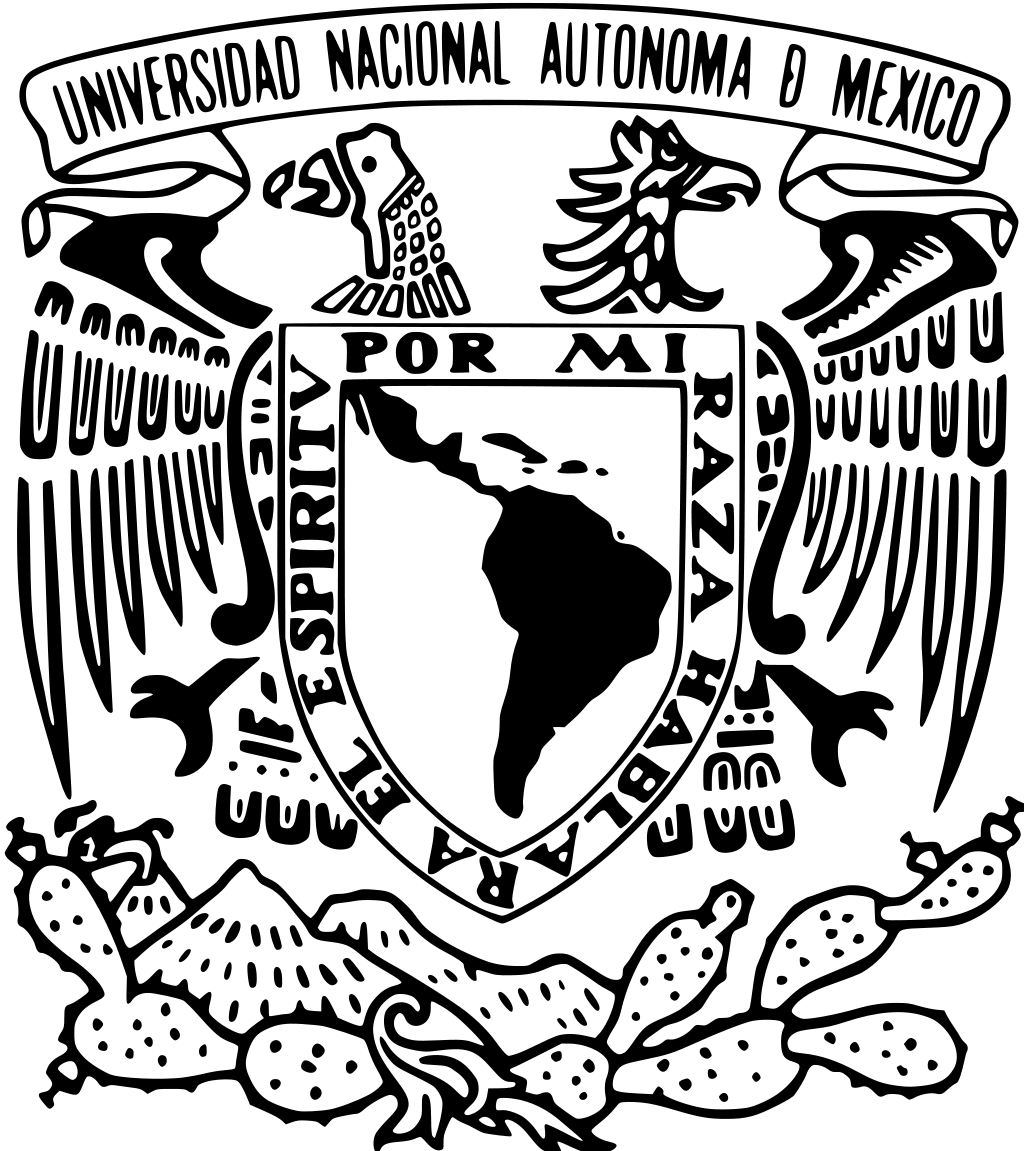
\includegraphics[width=0.2\textwidth]{../../unam.png}
        \vspace*{.5cm}

        \LARGE
        \textbf{Universidad Nacional Autónoma de México}

        \vspace{0.5cm}
        \LARGE
        Facultad de Estudios Superiores Acatlán

        \vspace{2cm}

        \textbf{Apuntes} \\
        Optimizacion 2

        \vfill

        \vspace{1cm}

        \textbf{\large Autor:} \\
        Jorge Miguel Alvarado Reyes \\
        \vspace{.5cm}
        \normalsize \today

    \end{center}
\end{titlepage}
\newpage

\tableofcontents

\newpage

\section{Problema 1}

Una fábrica de refrescos tiene plantas en la Cd. Mx., Toluca, Mérida, Cd. Juárez y Veracruz. Una fábrica de latas tiene plantas en Querétaro, Monterrey y Celaya. La demanda mensual de latas se pronostica en: Cd. Mx. 1 800 000; Toluca 800 000; Mérida 900 000; Cd. Juárez 300 000; y Veracruz 900 000. La producción mensual será: Querétaro 2 000 000; Monterrey 2 500 000; y Celaya 1 500 000. Los costos unitarios de flete son:

\begin{table}[h!]
    \centering
    \begin{tabular}{|l|c|c|c|c|c|}
        \hline
                           & \textbf{Cd. Mx.} & \textbf{Toluca} & \textbf{Mérida} & \textbf{Cd. Juárez} & \textbf{Veracruz} \\ \hline
        \textbf{Querétaro} & 25               & 15              & 35              & 80                  & 45                \\ \hline
        \textbf{Monterrey} & 30               & 45              & 85              & 50                  & 80                \\ \hline
        \textbf{Celaya}    & 20               & 15              & 40              & 40                  & 60                \\ \hline
    \end{tabular}
    \caption{Costos unitarios de flete}
\end{table}

\begin{enumerate}
    \item[(i)] Represente el problema en una gráfica bipartita.
    \item[(ii)] Proporcione una solución básica factible usando el método del costo mínimo.
    \item[(iii)] Determine la solución óptima.
    \item[(iv)] Interprete la solución dada en (iii) en términos de flujo en la gráfica (i).
\end{enumerate}

\end{document}